\section{Stmívaný LED pásek}
K budíku lze připojit LED pásek (ve firmware je tato funkce nazývána
\texttt{ambient}), který je pozvolna rozsvěcen před zahájením akustického
buzení. Cílem je simulovat postupné rozednění.

Na výstupu mikrokontroléru je PWM signál o frekvenci \SI{980}{\hertz}. % TODO overit, je to pin 6 Arduino. Jinak by byl 490Hz.
% https://www.arduino.cc/reference/en/language/functions/analog-io/analogwrite/
Přímé řízení samostatné výkonové LED či LED pásku tímto signálem by způsobovalo
blikání světla na této frekvenci. Proto je vhodnější plynule regulovat proud
protékající LED, která je napájena zdrojem konstantního proudu.

% TODO nevyhody PWM stmivani
% https://electronics.stackexchange.com/questions/277238/disadvantages-of-dimming-leds-via-current-regulation-as-opposed-to-via-pulse-fre


\subsection{Testovací verze -- lineární stmívač}
Pro prvotní ověření užitečnosti celého konceptu byl vytvořen jednoduchý
tranzistorový obvod, který slouží k napájení jedné LED o jmenovitém výkonu
\SI{1}{\watt} ze zdroje o napětí \SI{12}{\volt}. Obvod je určen pouze pro
testování a při jeho návrhu proto nebylo věnováno příliš pozornosti tomu, aby
byla závislost proudu protékajícího LED na střídě PWM signálu lineární (viz
graf na obrázku~\vref{fig:ambient linear napeti}).
Z tohoto důvodu není obvod vhodný pro použití ve finálním výrobku. Dalšími
nevýhodami jsou nízká účinnost, potřeba chladit výkonový tranzistor a z toho
vyplývající velké fyzické rozměry součástek. Obvod ale lze velmi snadno
sestavit na nepájivém kontaktním poli.

Výkonovou LED v pouzdře pro povrchovou montáž je nutné chladit, pro testování
prototypů lze využít výrobcem dodaný chladič. Jde o malou desku plošných spojů
s hliníkovým podkladem. Pro odvod tepla má LED na spodní straně plochu pro
připájení k chladiči. To znemožňuje pájení standardní mikropáječkou, spodní
strana totiž není přístupná. Vhodnější metodou je aplikování pájecí pasty
(tavidlo s obsahem pájky) a zahřátí celé desky na teplotu pájení. Pájení horkým
vzduchem by zbytečně tepelně namáhalo horní stranu LED (např. čočku), proto je
vhodnější aplikovat teplo ze spodní strany.

\begin{figure}[htb]
    \centering
    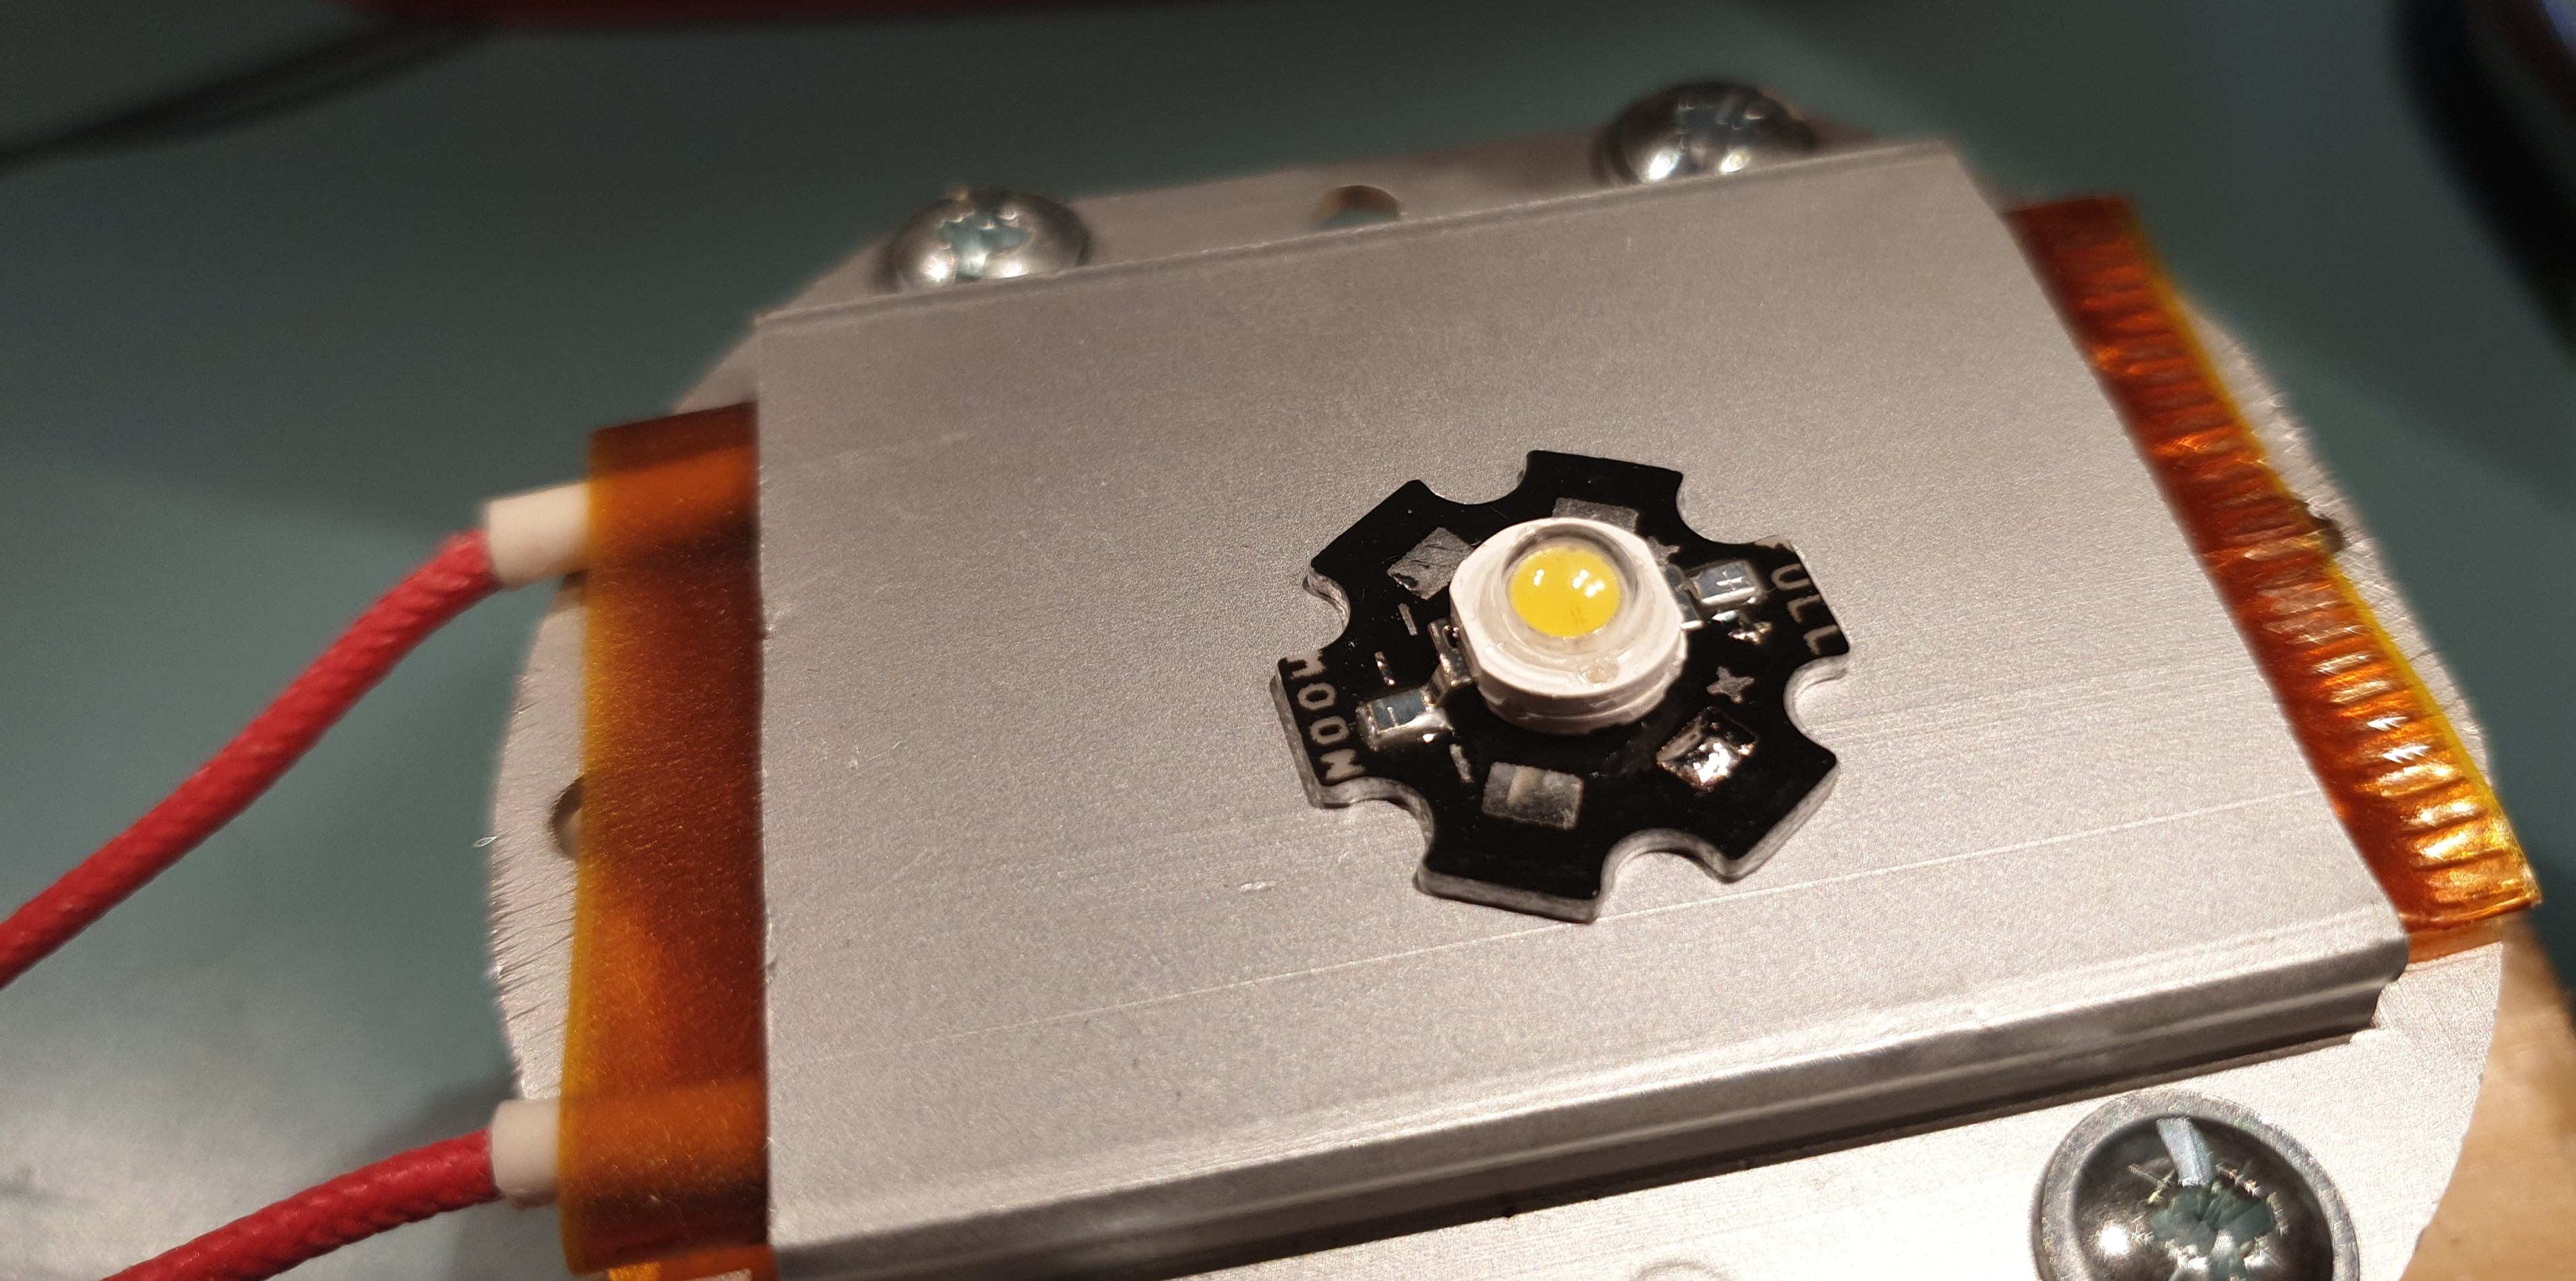
\includegraphics[width=0.5\textwidth]{ambient-LED-pajeni}
    \caption{Pájení výkonové SMD LED na chladič}
    \label{fig:ambient LED pajeni}
\end{figure}



\begin{figure}[htb]
    \centering
    \includegraphics[width=0.9\textwidth]{cropped_ambient-linear}
    \caption{Schéma zapojení testovacího lineárního stmívače pro výkonovou LED}
    \label{fig:ambient linear sch}
\end{figure}

Vstupní PWM signál je převáděn na analogové napětí dolní propustí (integračním
článkem RC tvořeným R1 a C1). Rezistory R2 a R3 určují střídu PWM
signálu, při které se LED začne rozsvěcet a kdy dosáhne plného jasu. Tranzistor
Q2 je použit kvůli nízkému proudovému zesilovacímu činiteli tranzistoru Q3, se
kterým tvoří darlingtonovo zapojení. Tranzistor Q3 reguluje proud protékající
LED (D1). Z důvodu poměrně velkého ztrátového výkonu na této součástce byl
použit tranzistor KUY12 v pouzdře TO-3. Rezistor R4 převádí proud protékající
větví s LED na napětí. Velikost odporu tohoto rezistoru určuje konstantní proud
při plném jasu, protože tranzistor Q1 na tomto rezistoru udržuje přibližně
konstantní úbytek napětí ($U_\mathrm{CE} \cong \SI{700}{\milli\volt}$).
Konstantní proud je tedy $I = \frac{U_\mathrm{CE}}{R_4} =
\frac{\SI{700}{\milli\volt}}{\SI{6,8}{\ohm}} \doteq \SI{103}{\milli\ampere}$.
Regulace probíhá přivíráním Q3.

\begin{figure}[htb]
    \centering
    \input{sim/graf-ambient-linear.tex}
    \caption{%
        Závislost proudu protékajícího LED diodou na napětí získaném filtrací
        PWM signálu na vstupu lineárního stmívače
        podle simulace v LTspice
    }
    \label{fig:ambient linear napeti}
\end{figure}
